\documentclass[journal]{IEEEtran}

% Additional packages
\usepackage{graphicx}
\usepackage{amsmath}
\usepackage{hyperref}
\usepackage{float}
\usepackage{subcaption}
\usepackage{booktabs}
\usepackage{pgfplotstable}
\usepackage{qrcode}

\pgfplotsset{compat=1.18}

\begin{document}

\title{Analysis of RLC Circuits: Serial and Parallel Configurations}
\author{IBRAHIM H.I. ABUSHAWISH \\
Istanbul University, Department of Physics \\
Instructor: Lect. Deniz Bozo\u{g}lu Parto \\
Experiment Date: 21.10.2024, Report Submission Date: 28.10.2024\\
Course \& Section Number: PHYS2305}

\maketitle

\begin{abstract}
This report presents a comprehensive analysis of RLC circuits, including serial and parallel configurations. It provides a detailed theoretical overview, experimental procedures, data analysis, and discussion of key findings. The analysis is supported by code-based calculations and graphical visualizations produced using Python.
\end{abstract}

\section{Introduction}
RLC circuits are fundamental in the study of alternating current (AC) electrical systems. They serve as essential components in filters, oscillators, and resonant circuits. This report aims to explore the behavior of both serial and parallel RLC circuits. Key objectives include analyzing the resonance phenomenon, calculating impedance, and visualizing phase shifts.

\section{Theory}

\subsection{Serial RLC Circuit}
A serial RLC circuit consists of a resistor (R), inductor (L), and capacitor (C) connected in series. The voltage applied across the circuit can be described as:
\begin{equation}
    U(t) = IR + L\frac{dI(t)}{dt} + \frac{Q}{C}
\end{equation}
where $U(t)$ is the applied voltage, $I(t)$ is the current, $R$ is the resistance, $L$ is the inductance, $C$ is the capacitance, and $Q$ is the charge on the capacitor. Solving for impedance $Z$, the following expression is obtained:
\begin{equation}
    Z = \sqrt{R^2 + \left(\omega L - \frac{1}{\omega C}\right)^2}
\end{equation}
The resonance frequency $f_0$ occurs when the impedance is minimal and is calculated as:
\begin{equation}
    f_0 = \frac{1}{2\pi \sqrt{LC}}
\end{equation}

\subsection{Parallel RLC Circuit}
A parallel RLC circuit has R, L, and C elements connected in parallel. The total impedance $Z$ is calculated as:
\begin{equation}
    \frac{1}{Z} = \frac{1}{j\omega L} + j\omega C + \frac{1}{R}
\end{equation}
The condition for resonance in a parallel RLC circuit is when the reactive components cancel each other, leading to:
\begin{equation}
    \omega_0 = \frac{1}{\sqrt{LC}}
\end{equation}

\section{Experimental Setup}
The experimental setup involves several essential components, including resistors, capacitors, and inductors, which are connected to form serial and parallel RLC circuits. An AC power source is used to provide alternating current, and measurements are taken using the Cobra3 PowerGraph software. The circuit diagrams for both serial and parallel RLC circuits are illustrated in Figures \ref{fig:serial_circuit} and \ref{fig:parallel_circuit}, respectively. 

\begin{figure}[H]
    \centering
    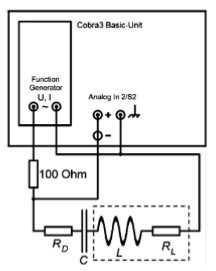
\includegraphics[width=0.5\linewidth]{IMAGES/series_diagram.png}
    \caption{Circuit diagram of a Serial RLC circuit.}
    \label{fig:serial_circuit}
\end{figure}

\begin{figure}[H]
    \centering
    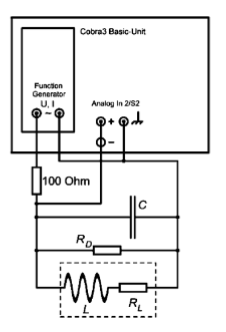
\includegraphics[width=0.5\linewidth]{IMAGES/parallel_diagram.png}
    \caption{Circuit diagram of a Parallel RLC circuit.}
    \label{fig:parallel_circuit}
\end{figure}

\section{Data and Calculations}
Data was collected for both serial and parallel RLC circuits. The key calculations performed are listed below:
\begin{itemize}
    \item Calculation of impedance as a function of frequency.
    \item Determination of resonance frequency for various RLC configurations.
    \item Calculation of the quality factor $Q$ for each configuration.
\end{itemize}

\subsection{Calculation of Resonance Frequency}
Using the equation for resonance frequency:
\begin{equation}
    f_0 = \frac{1}{2\pi \sqrt{LC}}
\end{equation}
The resonance frequency was calculated for each combination of L and C values. The calculated values are compared to experimental measurements.

\subsection{Graphical Analysis}
The following figures illustrate the relationship between impedance and frequency for both RLC circuit types.

\begin{figure}[H]
    \centering
    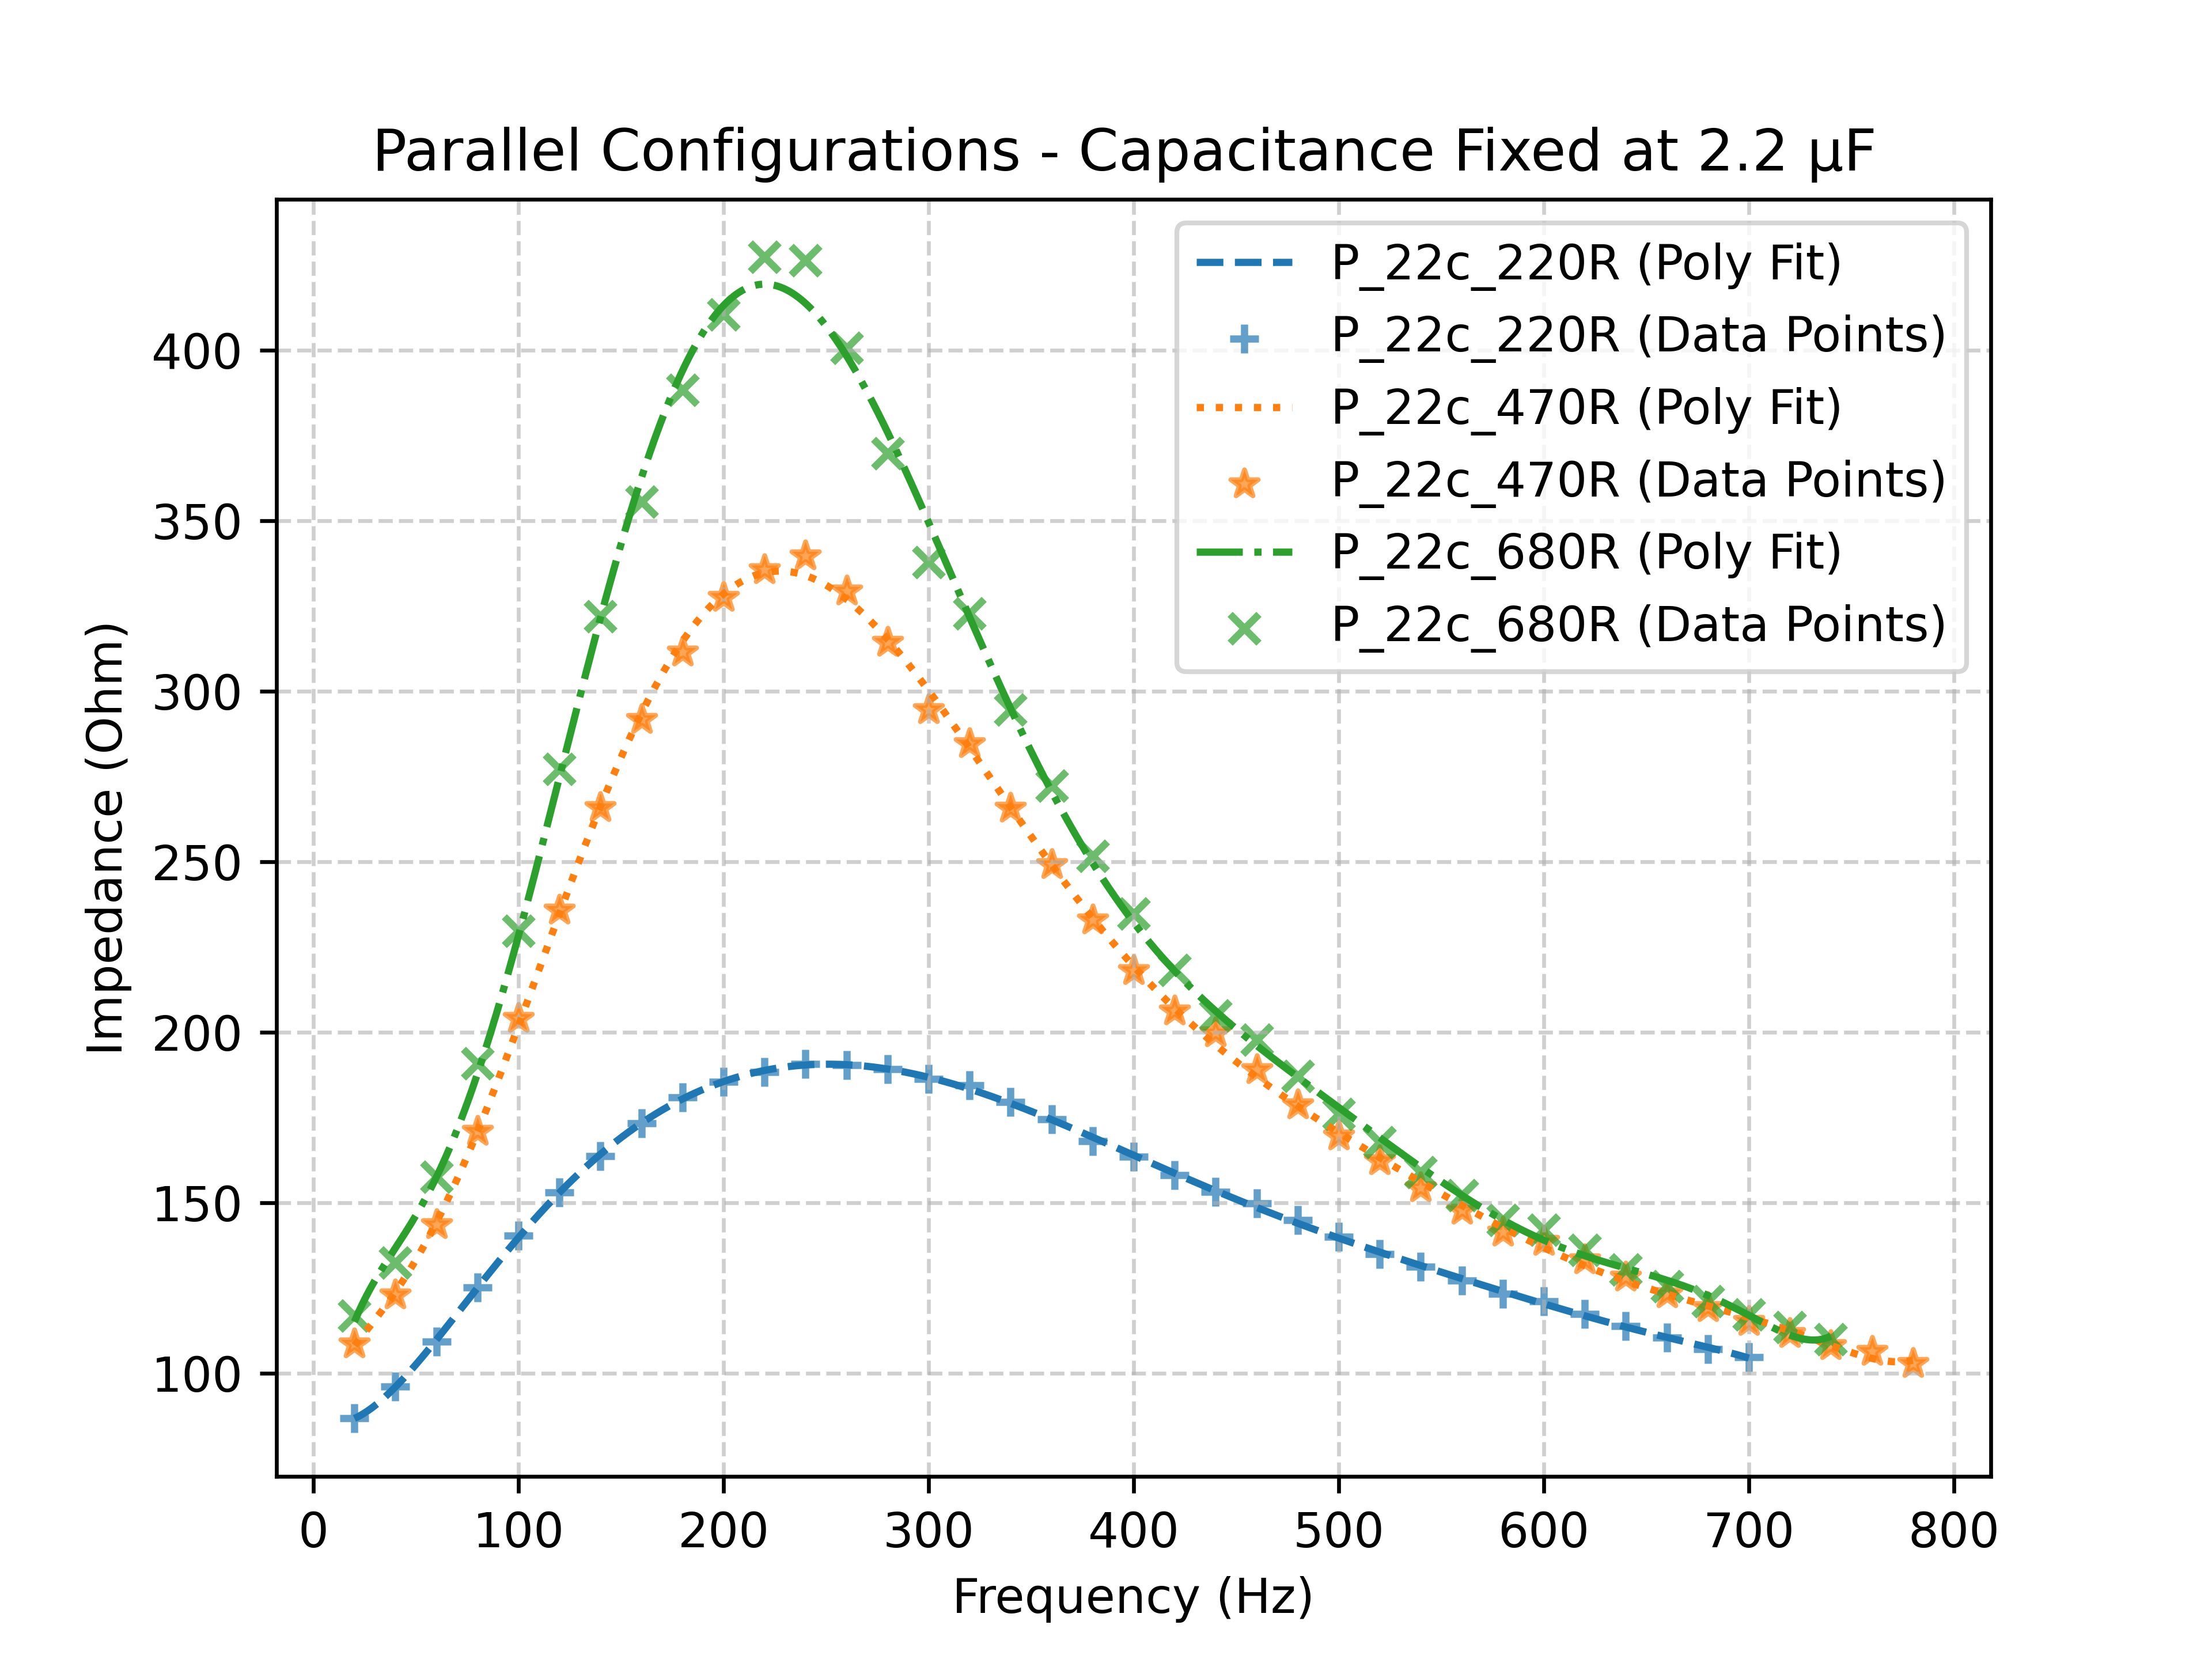
\includegraphics[width=\linewidth]{output_plots/Fixed_C/Parallel.png}
    \caption{Impedance as a function of frequency for serial and parallel RLC circuits.}
    \label{fig:impedance}
\end{figure}

\section{Results}
\subsection{Impedance vs. Frequency}
The plots in Figure \ref{fig:impedance} show how impedance varies with frequency. Resonance frequencies are clearly observed as points where the impedance is minimal.

\subsection{Quality Factor}
The quality factor $Q$ is calculated as:
\begin{equation}
    Q = \frac{f_0}{f_2 - f_1}
\end{equation}
where $f_1$ and $f_2$ are the half-power frequencies.

\section{Discussion}
The experimental results are compared to theoretical predictions. Deviations are analyzed, and sources of error such as measurement inaccuracies and component tolerances are identified.

\section{Conclusion}
This experiment provides a comprehensive understanding of RLC circuit behavior. Resonance, impedance, and phase shift were analyzed and validated with theoretical predictions.

\section*{References}
\begin{thebibliography}{1}
    \bibitem{example1} A. Author, \emph{Title of the Book}, 2nd ed. Location: Publisher, 2024.
    \bibitem{example2} B. Researcher, ``Title of the Article,'' \emph{Journal Name}, vol. 12, no. 3, pp. 45-67, 2023.
    \bibitem{example3} C. Scientist, \emph{Understanding RLC Circuits}, IEEE Press, 2022.
\end{thebibliography}

\appendices

\section{Python Code}
\begin{verbatim}
% Insert contents from Calculations.py
\end{verbatim}

\section{Lab Manual Excerpts}
\begin{verbatim}
% Insert relevant excerpts from PHYSICS_LAB_II-2.txt
\end{verbatim}

\end{document}
